\section{A straight-interpolation flow-matching oracle}
\label{supp:flow_oracle}

\begin{figure*}[t]
\centering
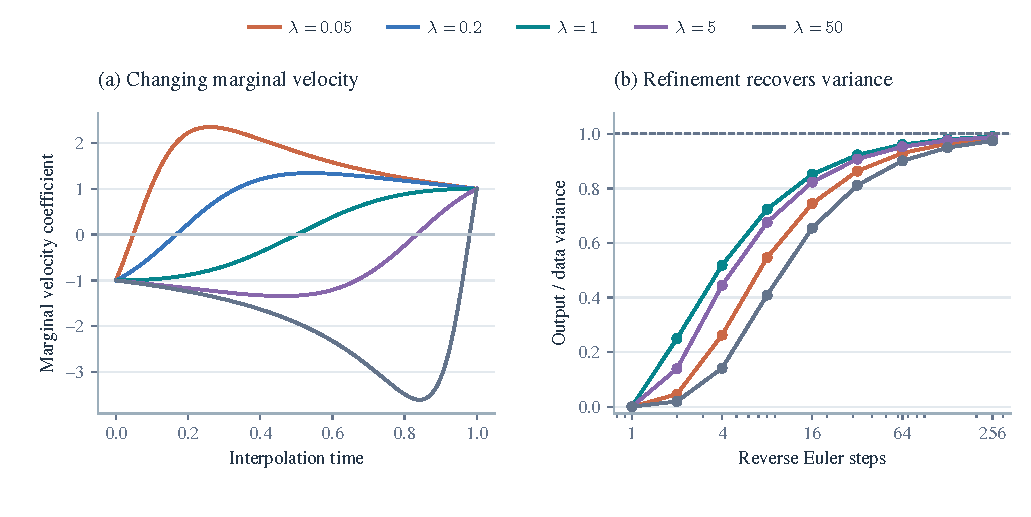
\includegraphics[width=\textwidth]{../figures/theory_flow.pdf}
\caption{Straight-interpolation Gaussian flow oracle. The population regression
velocity coefficient varies with time even though each endpoint-conditioned
path has a constant velocity. Reverse Euler sampling contracts the output
variance on the complete noise-to-data interval, and refinement approaches
the exact variance. Both panels show exact Gaussian-oracle predictions.}
\label{fig:flow_oracle}
\end{figure*}

A Gaussian oracle connects the same variance diagnostic to
straight-interpolation flow matching~\cite{lipman2023flow,liu2023rectified}.
To distinguish per-pair paths from the marginal sampling dynamics,
let $X_0\sim\mathcal N(0,\lambda)$ and $Z\sim\mathcal N(0,1)$ be independent,
with $\lambda>0$. For $t\in[0,1]$ from data to noise, define the
interpolated coordinate $X_t$ and its variance $v_t$:
\begin{equation}
X_t=(1-t)X_0+tZ,\qquad v_t=(1-t)^2\lambda+t^2.
\label{eq:fm_interpolation}
\end{equation}
The per-pair interpolation velocity $Z-X_0$ is constant. The population
regression field used by the marginal ODE at state $x$ is $b_t x$:
\begin{equation}
\mathbb E[Z-X_0\mid X_t=x]
=\frac{t-(1-t)\lambda}{v_t}x=b_tx.
\label{eq:fm_gaussian_velocity}
\end{equation}
This follows from Gaussian conditional expectation and
$\operatorname{Cov}(Z-X_0,X_t)=t-(1-t)\lambda$.
Because $b_t=\tfrac12\partial_t\log v_t$, exact ODE evolution from $t$ to $s$
maps $x_t$ to $\sqrt{v_s/v_t}\,x_t$. In particular, noise at $t=1$ reaches
variance $\lambda$ at $t=0$.

\paragraph{The measured variance ratio under Euler sampling.}
A reverse Euler step from $t$ to an earlier $s$ on a fixed descending grid multiplies a coordinate by
$m_{st}=1+(s-t)b_t$. Define
$u_t=((1-t)\sqrt\lambda,t)$, so that $v_t=\|u_t\|^2$. Since $u_t$ is affine,
\begin{equation}
m_{st}=\frac{u_s^\top u_t}{v_t}
=\sqrt{\frac{v_s}{v_t}}\cos\angle(u_s,u_t).
\label{eq:fm_euler_step}
\end{equation}
Let $X_{\rm out}$ be the final coordinate at $t=0$. Starting at $t=1$
with unit variance gives
\begin{equation}
\frac{\operatorname{Var}(X_{\rm out})}{\lambda}
=\prod_{t\rightarrow s}\cos^2\angle(u_s,u_t).
\label{eq:fm_variance_ratio}
\end{equation}
This is the same operational variance-ratio quantity as the Gaussian diffusion
calculation, derived here for explicit Euler on a different probability path.
For monotone grids spanning the fixed endpoints, the factors lie in $[0,1]$.
Refining an interval replaces $\cos^2(a+b)$ with
$\cos^2a\cos^2b$, which is no smaller for $a,b\geq0$, $a+b\leq\pi/2$.
The ratio converges to one as the maximum grid spacing vanishes.
At a truncated start with actual variance $\nu_{\rm start}$, an additional
factor $\nu_{\rm start}/v_{\rm start}$ appears, separating initialization from
integration as before.

For $\lambda=1$, four uniform reverse steps have multipliers
$(0.75,0.8,1,1.2)$, product $0.72$, and output variance $0.5184$.
A single full-interval Euler step has multiplier zero for every $\lambda>0$,
despite the straight per-pair interpolation paths. The supplied oracle script
checks five eigenvalues and nine grid sizes, and independently simulates
200,000 Gaussian samples for selected grids. It verifies the factorization
and monotone refinement numerically.

The oracle assumes independent Gaussian endpoints and an exact regression field.
Coupling is consequential: if instead $X_0=\sqrt\lambda Z$, one reverse Euler
step has multiplier $\sqrt\lambda$ and is exact. Straightness alone therefore
does not determine the sampling error; the marginal regression and endpoint
coupling matter. This is consistent with rectified flow's use of a changed
coupling to straighten marginal trajectories\cite{liu2023rectified}.
We use this elementary calculation to explain a measurable failure mode.
For learned flows, the empirical support, fidelity, and intervention checks
determine whether these effects predict useful repairs.

